% Chapter 2
\chapter{Descrizione generale} % Main chapter title
%----------------------------------------------------------------------------------------

% Define some commands to keep the formatting separated from the content 
% \newcommand{\keyword}[1]{\textbf{#1}}

%----------------------------------------------------------------------------------------
\section{Prospettiva del prodotto}

Il prodotto software sarà un sistema distribuito, basato su un'architettura client-server a tre livelli (presentazione, logica applicativa e dati), organizzata in due macro-componenti indipendenti: una parte di \textit{back-end}, che comprende la logica applicativa e la base di dati, e una di \textit{front-end}. 

\textbf{Back-end} \\
Avrà la responsabilità della gestione centralizzata dello stato del sistema, garantendo che tutte le informazioni e i dati persistenti siano conservati e aggiornati unicamente su di esso. Espone le proprie funzionalità tramite API REST e può essere eseguito in autonomia, senza dipendere da come è realizzato il front-end.

\textbf{Front-end} \\
Costituirà l'interfaccia utente realizzata come applicazione desktop, che si appoggerà esclusivamente ai servizi REST esposti dal back-end e potrà essere sostituita o modificata senza richiedere modifiche al back-end.

\section{Funzioni del prodotto}
In questo paragrafo sono stati elencati i requisiti funzionali utente, dedotti dalle funzionalità descritte nel primo capitolo, e descritti mediante i diagrammi di caso d'uso.
Il paragrafo è suddiviso in due parti:

\begin{quote}
Nella \textit{prima parte} verrà fornito un elenco dei requisiti funzionali dedotti, espressi in modo comprensibile anche per gli utenti senza un'approfondita conoscenza tecnica.     
\end{quote}

\begin{quote}
Nella \textit{seconda parte} verranno presentati i diagrammi di caso d'uso, i quali saranno associati a uno o più requisiti.
\end{quote}

\subsection{Requisiti funzionali utente}
\begin{quote}
\begin{enumerate}[label=\textit{RF\arabic*}]
  \item \textbf{Il sistema deve offrire un meccanismo di autenticazione.}
    
  \item \textbf{Il sistema deve poter permettere a ogni account \textit{Amministratore} di creare ulteriori utenti, sia normali che di tipo amministratore, specificando le loro credenziali di accesso. }
  
  \item \textbf{Gli utenti possono segnalare issue, con la possibilità di specificare un titolo, una descrizione, una priorità, una immagine e il tipo.}
  
  \item \textbf{Il sistema deve permettere la visualizzazione di tutte le issue segnalate, con la possibilità di filtrare e ordinare i risultati.}
  
  \item \textbf{Il sistema deve permettere, solo a un \textit{Amministratore}, di assegnare bug e notificare un membro del team.}
  
  \item \textbf{Il sistema deve consentire a un \textit{utente normale} di ricevere notifiche riguardanti i bug.}

  \item \textbf{Ogni \textit{utente normale} può visualizzare i propri bug assegnati.}

  \item \textbf{Il sistema deve fornire una funzione di ricerca per trovare issue.}

  \item \textbf{Il sistema può suggerire automaticamente a chi assegnare un bug.}
  
\end{enumerate} 
\end{quote}

\subsection{Diagrammi di caso d'uso} 

Qui di seguito vengono illustrati i diagrammi di caso d'uso che modellano i requisiti sopra citati.

\begin{figure}[!ht] 
\begin{center}
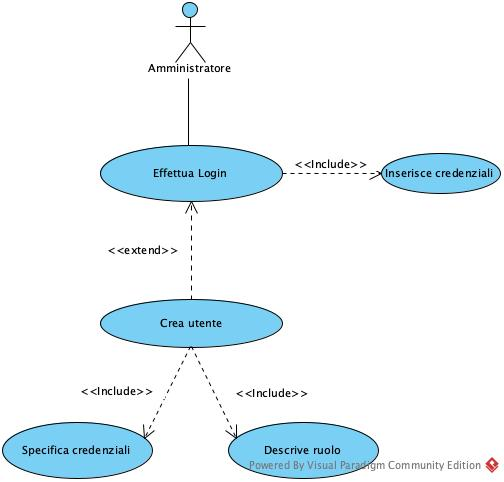
\includegraphics[width=10cm]{Chapters/Punto1.jpg}
\end{center}
\caption{Modellazione requisiti \textit{RF1}, \textit{RF2}}
\label{fig:f1} 
\end{figure}

\begin{figure}[!ht] 
\begin{center}
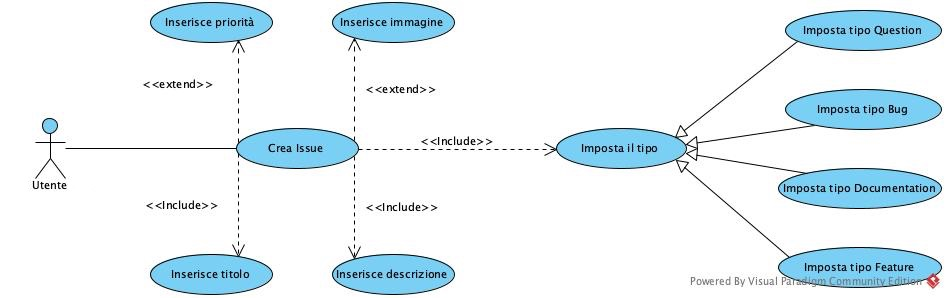
\includegraphics[width=15cm]{Chapters/Punto2.jpg}
\end{center}
\caption{Modellazione requisito \textit{RF3}}
\label{fig:f2} 
\end{figure}

\begin{figure}[!ht] 
\begin{center}
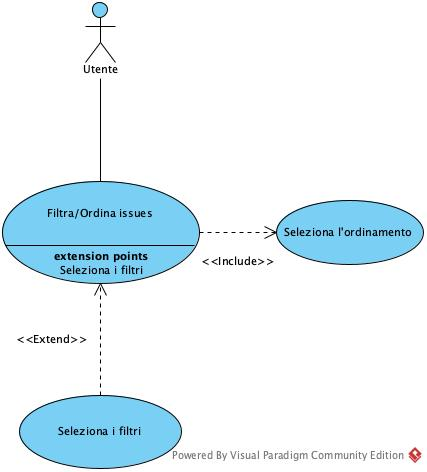
\includegraphics[width=10cm]{Chapters/Punto3.jpg}
\end{center}
\caption{Modellazione requisito \textit{RF4}}
\label{fig:f3} 
\end{figure}

\begin{figure}[!ht] 
\begin{center}
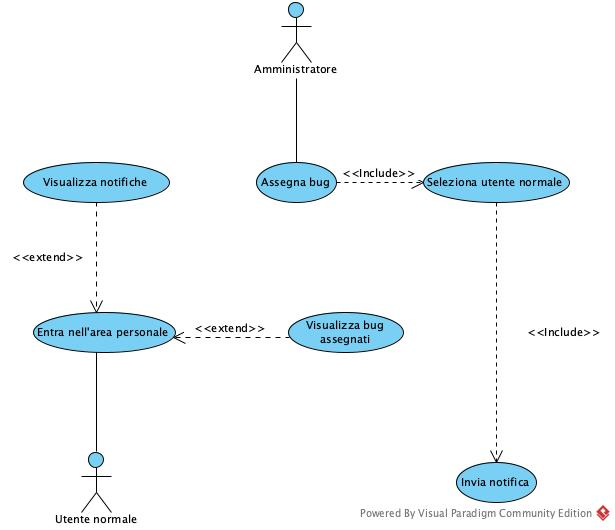
\includegraphics[width=12cm]{Chapters/Punto4.jpg}
\end{center}
\caption{Modellazione requisiti \textit{RF5}, \textit{RF6}, \textit{RF7}}
\label{fig:f4} 
\end{figure}

\begin{figure}[!ht] 
\begin{center}
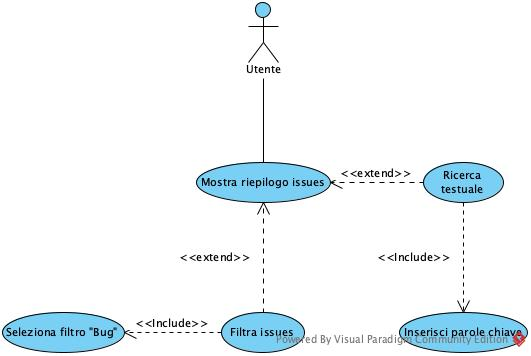
\includegraphics[width=12cm]{Chapters/Punto11.jpg}
\end{center}
\caption{Modellazione requisiti \textit{RF4}, \textit{RF8}}
\label{fig:f5} 
\end{figure}

\begin{figure}[!ht] 
\begin{center}
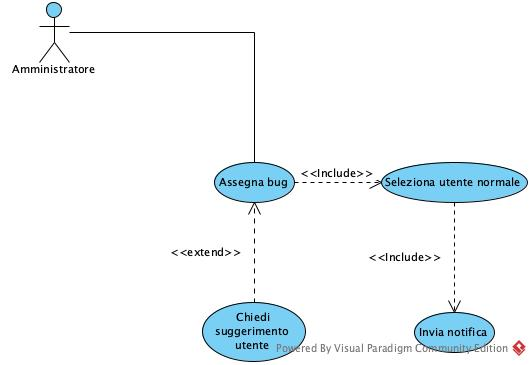
\includegraphics[width=15cm]{Chapters/Punto14.jpg} 
\end{center}
\caption{Modellazione requisiti \textit{RF5},\textit{RF9}}
\label{fig:f6} 
\end{figure}

% \begin{figure}
%     \centering
%     
\includegraphics[width=.6\textwidth]{Dedication/dedication.pdf}
%     \caption{An example dedication page.}
%     \label{fig:chap2:dedication_sample}
% \end{figure}


\clearpage

\section{Caratteristiche utente}
L'utilizzo di BugBoard26 richiede che gli utenti, membri di un team di sviluppo, abbiano una buona conoscenza del dominio applicativo del progetto su cui lavorano. Devono saper riconoscere un problema, descriverlo con chiarezza e scegliere il tipo di issue corretto (bug, documentazione, feature o domanda). \\
\indent Una segnalazione imprecisa porta infatti a perdite di tempo e fraintendimenti.
Tutti gli utenti, dopo l'autenticazione, possono segnalare issue e consultarle tramite la vista riepilogativa. In base al ruolo ricoperto, si distinguono due categorie:

\textbf{Amministratore}\\
È l'utente con privilegi di gestione. Crea nuovi utenti, normali o amministratori, e gestisce i bug: li assegna ai membri del team, aiutato dai suggerimenti del sistema basati sul carico di lavoro, li contrassegna come duplicati e chiude le issue. Non riceve bug assegnati né notifiche.

\textbf{Utente normale}\\
È l'utente senza privilegi di gestione e corrisponde agli sviluppatori del team. Oltre a segnalare problemi e proporre nuove funzionalità, può ricevere l'assegnazione di bug, consultarli in un'apposita sezione e ricevere notifiche sulle assegnazioni e sulle chiusure dei bug che gli sono stati assegnati.

\section{Presupposti e dipendenze}

\subsection{Dipendenze tecnologiche}
\begin{itemize}
  \item \textit{Containerizzazione del back-end}: come auspicato dal committente, il back-end viene distribuito come immagine \textit{Docker}, insieme a un file \textit{Docker Compose} che avvia sia il back-end sia la base di dati.

  \begin{itemize}
  \item \textit{Dipendenze}: Si assume che la macchina server disponga di un demone \textit{Docker} correttamente installato e configurato.
\end{itemize}
\end{itemize}
\begin{itemize}
  \item \textit{Base di dati}: il back-end memorizza i dati persistenti in un database MySQL.
  \begin{itemize}
  \item \textit{Dipendenze}: con Docker Compose il database viene avviato automaticamente e il back-end parte solo quando il database è pronto. Se il back-end viene eseguito senza Docker, si assume che sia disponibile un server MySQL raggiungibile.
\end{itemize}
\end{itemize}

\subsection{Dipendenze sull'ambiente dell'utente}
\begin{itemize}
  \item \textit{Ambiente di esecuzione del client}: il front-end è un'applicazione desktop.  \begin{itemize}
  \item \textit{Dipendenze}:si assume che sulle macchine degli utenti sia installato un ambiente Java compatibile con il front-end.
\end{itemize}
\end{itemize}

\begin{itemize}
  \item \textit{Connettività di rete}: L'architettura di sistema prevede 
  che il \textit{front-end} comunichi con il \textit{back-end} esclusivamente tramite le API REST, anche 
  quando quest'ultimo risiede in una rete esterna.
  \begin{itemize}
  \item \textit{Dipendenze}: Si assume che il back-end sia raggiungibile dalle macchine degli utenti. Se le due parti si trovano su reti separate, gli utenti devono disporre di una connessione Internet stabile, perché la qualità dell'esperienza d'uso dipende dalle prestazioni della rete.
\end{itemize}
\end{itemize}
